\chapter[Background information]{Background information} \label{ch:background}

The first phase of the CRISP-DM process model for data mining projects is business understanding;
this chapter discusses the complex interaction of land use and transportation, provides a brief overview of the history of development of land use and transportation (LUT) models, presents some legal and historical background for Teranet's dataset of land registration records, and finishes with a discussion of challenges of working with Teranet's data and the proposed solution.

\section{Complexity of urban systems and ``wicked'' problems} \label{sec:complexity_and_wicked_problems}

In her famous 1961 book, Jane Jacobs\cite{Jacobs1961} described a city as "a problem in organized complexity";
since then, many other researchers have remarked that urban systems exhibit complex behaviour\cite{Batty2008, Bettencourt2013}.
Complexity of a system can be defined as a state or quality of being intricate or complicated.
For a system to be complex is not necessarily the same as to be complicated;
complex systems can be simple, i.e.\ governed by a single equation.
Complexity of a system has to do with the intrinsic ability of a system to surprise us with its behaviour;
that the system is hard to understand, despite the mechanics of it being relatively simple.

In 1973, a little over a decade after Jacobs, Rittel and Webber\cite{Rittel1973} presented a path-breaking conceptualization;
this conceptualization characterized urban planning problems as ``wicked'' problems: problems which cannot be definitively described and for which it makes no sense to talk of ``optimal solutions''.
In their paper, Rittel and Webber stated that such ``wicked'' problems are never ``solved'', and that the focus instead becomes on iteratively ``re-solving'' the problems over and over.
More than 40 years after their original publication, Rittel and Webber's ideas remain relevant to the policy sciences today: there is an intense interest in the nature of ``wicked'' problems and the complex tasks of identifying their scope, viable responses, and appropriate mechanisms and pathways to improvement\cite{Crowley2017}.
Interaction between land use and transportation, which is discussed in the following section, presents a prime example of urban complexities and ``wicked'' problems.

\section{Transportation-land use cycle} \label{sec:transportation_land_use_cycle}

Among the reasons why transportation and land use interaction is ``wicked'' are such aspects as pluralism of expectations among stakeholders, institutional complexity in policy making, and scientific uncertainty\cite{Noto2015}.
More importantly, there is a fundamental link between transportation and urban form: urban form has an enormous impact on the type and cost of transportation systems needed to serve residents of a metropolitan area\cite{Kelly1994}.
Transportation, in turn, influences land development and location choices of people and firms, and thus completes the formation of a feedback relationship that Stover and Koepke\cite{Stover1988} referred to as a cycle.
Interconnections between points (activities) in space can be perceived through the medium of the transportation system\cite{Miller1998}

Figure~\ref{fig:idealized_integrated_urban_model} illustrates the complex interactions between land use and transportation system as summarized by Miller, Kriger and Hunt\cite{Miller1998}.

\begin{figure}[hbt!]
    \centering
    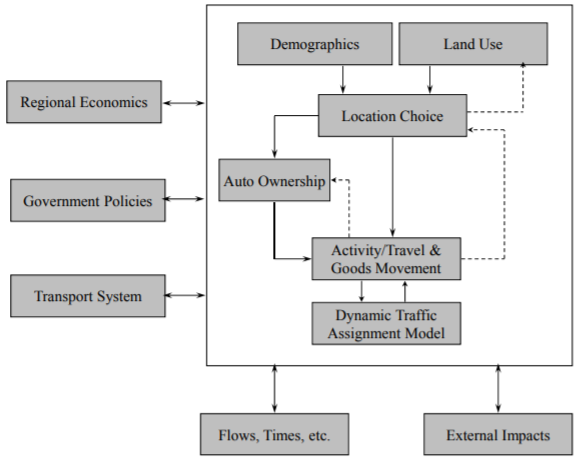
\includegraphics[width=0.7\linewidth,trim=0 0 0 0,clip]{miller_idealized_urban_model.png}
    \caption{An Idealized Integrated Urban Model System, adapted from Miller, Kriger and Hunt\cite{Miller1998}.}
    \label{fig:idealized_integrated_urban_model}
\end{figure}

Many different types of models are used in planning, such as demand forecasting models projecting traffic or ridership, or land use models projecting and distributing population and jobs within an area.
At an earlier stage of model development, some analysts argued that there is no significant link between transportation and land use, given the near-ubiquity of the transportation (road) network\cite{Miller1998}.
However, the unprecedented urban growth of the 21st century introduced new challenges for urban systems such as extreme road congestion, equity of access to jobs and services among low-income households, energy scarcity, environmental and GHG impacts from transportation systems and public health impacts of land use patterns\cite{Miller2018b,Moeckel2017}.

It became apparent that these ``transport problems'' cannot be solved through transportation policies and investment alone, that the physical design of the city at the ``macro'' and ``micro'' scale critically interfaces with the demand for and performance of the transportation system.
In addition, to accurately assess the costs and benefits of an expensive long-term transportation infrastructure investment, ``feedback'' effects of these investments on urban form, land values, property taxes, quality of life, etc.
need to be quantified and included in evaluation and decision making.
Thus, today there is a steadily growing recognition within the urban policy field that the interaction between transportation and land use does exist and does matter\cite{Miller2018b}.

In the context of models, integrated urban models (IUMs) aim to capture the complex relationship between urban systems such as transportation and land use more accurately.
Integrated land use-transportation models combine travel demand forecasting and land use forecasting functions and recognize that the distribution of population and jobs depends, in part, on transportation accessibility.
The reverse is also true, and thus integrated models incorporate feedback relationship between transportation and land use, with economic decisions by households and firms acting as one of the links between the two systems\cite{Miller1998}.

\section{Evolution of LUT models} \label{sec:evolution_of_lut_models}

The history of treating cities as systems via simulation models of transportation and land use dates back to the 1950s when General System Theory and Cybernetics came to be applied in the softer social sciences\cite{Batty2008}.
The first operational simulation model that truly integrated land use and transportation is considered to be A Model of Metropolis built in 1964 by Ira S. Lowry for the Pittsburgh region based on economic base theory\cite{Lowry1964}.
It was a highly aggregate model based on theories of spatial interaction, such as the gravity model that was popular in quantitative geography and transportation planning at the time\cite{Bouchard1965}.
Models based on a spatial interaction framework continued to be developed through mid-1980s, until developments in random utility theory allowed researchers to describe choices among discrete alternatives, such as the choice of travel mode, and generate models based on the study of disaggregate behaviour\cite{Iacono2008}.

Figure~\ref{fig:lut_model_evolution} provides the general overview of chronological development of LUT models as summarized by Iacono\cite{Iacono2008}.

\begin{figure}[hbt!]
    \centering
    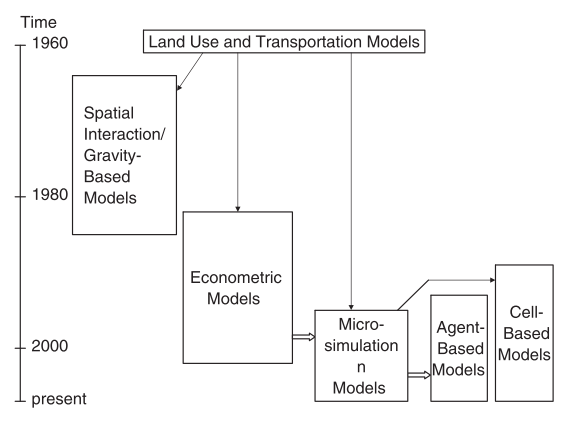
\includegraphics[width=0.7\linewidth,trim=0 0 0 0,clip]{lut_models_evolution.png}
    \caption{Chronological development of LUT models as summarized by Iacono\cite{Iacono2008}.}
    \label{fig:lut_model_evolution}
\end{figure}

The modeling paradigm changed fundamentally in the early 1990s along with the advances in computing power and efficiency of data storage.
Urban systems used to be viewed as hierarchical and centrally organized equilibrium structures, or ``top-down''.
Instead, now they were considered to be structured from the ``bottom-up'', dynamically retaining their integrity through interactions of numerous microelements\cite{Batty2008}.
A new broad class of LUT models that could fall under the title of ``microsimulation'' began to be developed: these included such classes of models as activity-based travel, cell-based models, multi-agent models, and more recently comprehensive urban microsimulation models that reflect the dynamics of changes in the population and the urban environment\cite{Iacono2008}.
``Micro'' in the microsimulation implies that the model must be highly disaggregated spatially, socio-economically and in its representation of processes.
``Simulation'' implies that the model must be numerical, stochastic, have an explicit time dimension, and ``evolve'' into the end state rather than ``solve for it''\cite{Miller2019}.
An example of such a model has been developed by the University of Toronto ILUTE team;
their product is an integrated urban model capable of microsimulating urban demographic evolution, housing markets and travel behaviour over extended periods of time\cite{Miller2018a}.

The Integrated Land Use, Transportation, Environment (ILUTE) model system is a system of disaggregate agent-based microsimulation models for Greater Toronto--Hamilton Area (GTHA).
It includes such components as land use, activity/travel, urban economics, auto ownership, demographics and emissions/energy use.
The system uses disaggregate models of spatial socioeconomic processes to evolve from a known base case to a predicted end state of the GTHA in 1-year time steps\cite{Miller2011}.
In ILUTE, the system state of GTHA is defined in terms of the individual persons, households, dwelling units, firms, etc.
that collectively define the urban region being modeled.
Many markets are of interest within ILUTE, such as housing, labour, commercial, real estate, etc., and are modeled via microsimulation.
For example in HoMES, the housing market module of ILUTE, houses are auctioned off one dwelling at a time to interested bidders in a disaggregate implementation of Martinez' Bid Choice theory\cite{Rosenfield2013,Martinez1992}.

Among the major barriers to implementation of integrated urban models since their introduction were such aspects as data hungriness and computational requirements\cite{Miller1998}.
However, as an increasing amount of aspects of human life becomes digitalized, a wealth of new data is produced and can be used to model and analyze dynamics of urban systems\cite{Arribas-Bel2014,Chen2016}.
Furthermore, continuing methodological advances in computing, such as cost-effective High Performance Computing (HPC), detailed GIS-based datasets and machine learning methods, mean that former barriers now represent opportunities for model system development\cite{Miller2018a}.
An example of such digitalization of human activity is the introduction of the Province of Ontario Land Registration Information System (POLARIS) in 1985 by the Government of Ontario\cite{TeranetEnterprisesInc.}.
Introduction of POLARIS lead to a complete digitization of land registration records which in turn allowed the creation of an extensive dataset of real estate transactions by the Teranet Enterprises Inc.
Due to its high spatial and temporal resolution, Teranet's dataset holds a wealth of information about Ontario's housing market from 1985 to 2017 and thus presents a valuable resource to inform and validate the design of ILUTE and HoMES.
In addition, Teranet's dataset plays an important part in the Longitudinal Housing Market Research conducted by UTTRI which is discussed in the following section.

\section{Longitudinal Housing Market Research conducted by UTTRI} \label{sec:longitudinal_housing_market_research}

There is ample evidence of the role of land use and transportation interactions in determining urban spatial structure.
Accessibility and mobility provided by transportation systems drive economic development and impact travel behaviour and location of households and firms.
Similarly, urban sprawl and location of activities drive travel demand and the need for building transport networks.
Land values in a metropolitan region are an outcome of such land use-transportation interactions.

Researchers at the University of Toronto Transportation Research Institute are conducting longitudinal analysis to identify trends and changes in land value distributions using the Teranet sales data over the 30-year period (1986-2016) in the Greater Toronto-Hamilton Area (GTHA).
The aim is to understand the spatial-temporal effects of changes in socio-economic characteristics, transportation accessibility and built-environment on land values.
Data from various sources (e.g., Census, Transportation Tomorrow Survey, etc.) is required to be merged at the land parcel level to enhance datasets with additional attributes, while maintaining the ease of data storage and retrieval for analysis as needed.
In addition to that, accurate land use information needs to be added to Teranet records to allow separating sales data by major property types.

A brief legal and historical background of Teranet's dataset, main challenges of working with it and the proposed solution are discussed in the remainder of this chapter.

\section{POLARIS: electronic system of land registration in Ontario} \label{sec:polaris}

All land owned in Canada is registered in a public land registry in the applicable province.
Each province and territory in Canada has its own land registry system, whether it is a land titles system, a registry system or a combination of both, with each system having its own rules.
The registry system is a public record of documents evidencing transactions affecting land.
In the land titles system, the applicable provincial government determines the quality of the title, and essentially guarantees (within certain statutory limits) the title to, and interests in, the property.
As of 2015, most common law provinces and territories in Canada were using the land titles system or were in the process of converting from a registry system to a land titles system\cite{McKean2015}.

As of 2015, the Province of Ontario has largely converted from registry systems to a land titles system.
In 1985, the Government of Ontario initiated the Province of Ontario Land Registration Information System (POLARIS) pilot project for the purposes of the conversion between systems and records automation.
The Land Registration Reform Act (Ontario)\cite{TheGovernmentofOntario1990} was introduced in 1990 to facilitate electronic search and registration of properties and the automation of paper-based records.
POLARIS was built by the Province to house and process electronic land records, which in turn lead to the creation of an extensive dataset of land registration records managed by Teranet Enterprises Inc.
Today, POLARIS is the search/registration and property maintenance system for all automated land records in Ontario.

\section{Teranet's dataset, its challenges and the proposed solution} \label{sec:teranet_challenges_solution}

In 1991, the Government of Ontario established a partnership with Teranet, a Toronto-based organization, founded the same year, which provides e-services to legal, real estate, government, financial, and healthcare markets.
The partnership was established to convert Ontario's land registration system to a more modernized electronic title system.
The project involved taking a 200-year-old paper-based system and creating a database with electronic records for more than five million parcels of land.
Teranet converted all qualified Registry properties in Ontario to the Land Titles system and automated existing paper Land Titles parcels.
As a result, 99.9\% of property in Ontario was parcelized and administered under the Land Titles system.
Teranet fully automated the conversion of millions of paper-based documents and records into the Ontario Electronic Land Registration System (ELRS)\cite{TeranetEnterprisesInc.2019}.
Figure~\ref{fig:teranet_dmti_lu} presents an example of Teranet data: records from 2014 that fall within 1,000m of an arbitrarily selected target point, colored by land use spatially joined from DMTI datasets.

\begin{figure}[hbt!]
    \centering
    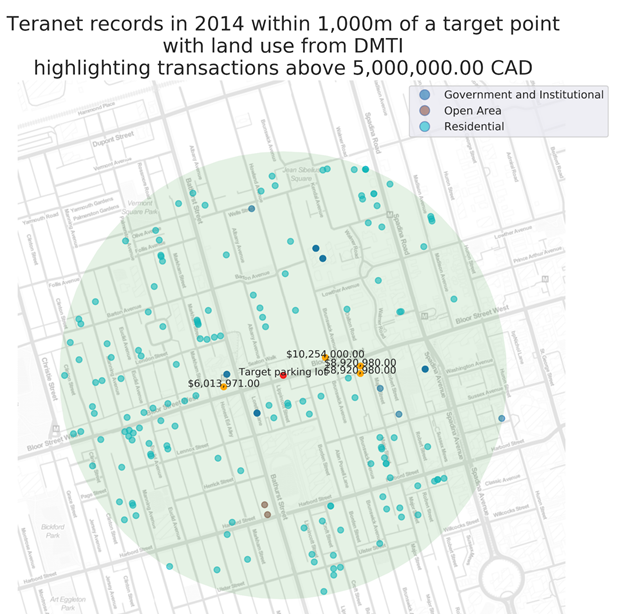
\includegraphics[width=0.8\linewidth,trim=0 0 0 0,clip]{teranet_dmti_lu.png}
    \caption{A sample map from Teranet dataset: records from 2014 within 1,000m of an arbitrarily selected target point, colored by land use spatially joined from DMTI datasets.}
    \label{fig:teranet_dmti_lu}
\end{figure}

Teranet's dataset presents an extensive historical record of real estate transactions recorded in the Province of Ontario since the beginning of the nineteenth century.
However, its available version also suffers from severe lack of features describing each transaction, which makes meaningful analysis or modeling difficult.
At the same time, each Teranet transaction has a timestamp (date) and location information (x and y coordinates) and thus can be joined to variety of other geocoded urban data sources, such as Census demographics, Transportation Tomorrow Survey (TTS) and parcel-level land use information.
However, joining these data sources together requires additional considerations, as they use different spatial units and are available at different temporal spans, as will be discussed in chapter~\ref{ch:spatial_and_temporal_relationships}.

One of the major attributes missing from the available version of Teranet's dataset is the information about the type of property being transacted, with records from various categories of residential, commercial and industrial properties all being mixed together in the same dataset.
This introduces a major limitation on how Teranet's data can be used, limiting the ability to separate the transactions of different property types, identify submarkets of the housing market and see its fine-scale characteristics and dynamics.
Detailed parcel-level land use information could offer some degree of filtering and can be joined from such sources as DMTI Spatial's land use and detailed land use manually collected by the Department of Geography at the University of Toronto.

\vspace{5mm}

However, these sources of land use information also have their limitations:
\begin{itemize}
    \item DMTI's land use data does not offer any split between subcategories of residential properties and only covers the period of 2001--2014
    \item land use from the Department of Geography is much more detailed and accurate, but has been collected at a single point in time over the summer of 2012 and 2013
    \item neither of the available land use sources covers the full span of the Longitudinal Housing Market Research conducted by UTTRI (1986-2016)
\end{itemize}

At the same time, detailed land use from the Department of Geography offers an opportunity to train a machine learning model capable of recognizing certain property types that have characteristically different behavior on the housing market (e.g., high / low volume of transactions, median price ratio, etc.).
Teranet records coming from a particular parcel (x and y coordinate pair) or pin (same parcel can include different pins, i.e.\ apartment complexes) can be combined to produce new features that characterize the behavior of this parcel or pin on the housing market.
Combining these new features with spatially-joined variables from Census and TTS can yield a dataset that can be used to train and test a classification algorithm capable of determining the parcel land use based on the nature of its behavior on the housing market at Teranet transaction level (recognizing changes of land use with time).

\vspace{5mm}

The primary focus of this thesis consists of:

\begin{itemize}
    \item augmenting Teranet's dataset with TTS, Census and land use variables, while maintaining the integrity of the spatial and temporal relationships between different data sources and ensuring the ease of storage and retrieval as needed for the Longitudinal Housing Market Research conducted by UTTRI
    \item investigating the opportunity for the implementation of a machine learning algorithm to classify land use based on the housing market dynamics
\end{itemize}

\section{Chapter summary} \label{sec:background_summary}

The complex interaction of land use and transportation has been treated via simulation models since 1950s.
Over the decades, the modeling paradigm has evolved from the highly aggregated and ``top-down'' representations of processes, such as gravity-based models, to highly disaggregated and ``bottom-up'', defining the macro state of the system through countless interactions of its microcomponents.
These changes are represented in the family of microsimulation models which can define the state of an urban region in terms of the individual persons, households, dwelling units, firms, etc.\ and evolve from a know base case into a future state via simulation.

It also became more clear with time that land use and transportation systems are deeply interconnected, and thus must be modeled together to incorporate feedback relationship, as is attempted by integrated urban models.
An example of the class of integrated microsimulation urban model systems, Integrated Land Use, Transportation, Environment, or ILUTE, model system has been developed at the University of Toronto for the Greater Toronto--Hamilton Area.

Since their introduction, among the major barriers to the implementation of integrated models were their data hungriness and computational requirements.
However, continuing methodological advances in computing expand modeling capabilities and increased digitization of human activity creates new datasets with spatial and temporal resolution that was not available before.
Together, these developments present opportunities for further improvement and validation of ILUTE and its modules.

An example of new emerging data sources is Teranet's dataset of real estate sales that was created after the introduction of POLARIS land registration system by the Province of Ontario in 1985.
Teranet's dataset plays an important part in the Longitudinal Housing Market Research conducted by UTTRI .
One of the major challenges of working with Teranet's data is the lack of features describing each transaction, namely the type of property being sold.
As Teranet's records have timestamps (dates) and coordinates of parcel centroids for each record, they can be joined with other data sources via temporal and spatial relationships;
nature of this relationships will be discussed further in chapter~\ref{ch:spatial_and_temporal_relationships}.
